\jxhj{%教学后记
	}
\skrq{%授课日期
	2017年10月10日 4-5节}
\ktmq{%课题名称
	 刀具半径补偿的应用(一)}
\jxmb{%教学目标,每行前面要加 \item
	\item 掌握用刀补进行精加工;
	\item 掌握刀补值的计算;
	\item 会用G41/G42刀具半径指令编写程序;
	\item 了解常用切入切出的方法。
 }
\jxzd{%教学重点,每行前面要加 \item
	\item 用刀补进行精加工;
	\item 刀补值的计算。 }
\jxnd{%教学难点,每行前面要加 \item
	\item 刀补值的计算。 }
\jjff{%教学方法
	通过讲述、举例、演示、分析法来说明;}

\makeshouye %制作教案首页

%%%%教学内容
\subsection{组织教学}
\begin{enumerate}[\hspace{2em}1、]
	\item 集中学生注意力;
	\item 清查学生人数;
	\item 维持课堂纪律;
\end{enumerate}
\subsection{复习导入及主要内容}
\begin{enumerate}[1、]
\item 刀补的概念
\item G40、G41/G42指令的使用;
\item 注意事项;
\item 刀补的编程;
\item 在数控铣床或加工中心上加工如图\ref{fig:8-1}所示的零件,试完成程序的编写。(试用I、J、K编写,凸台高5mm)

\begin{figure}[h]
	\centering
	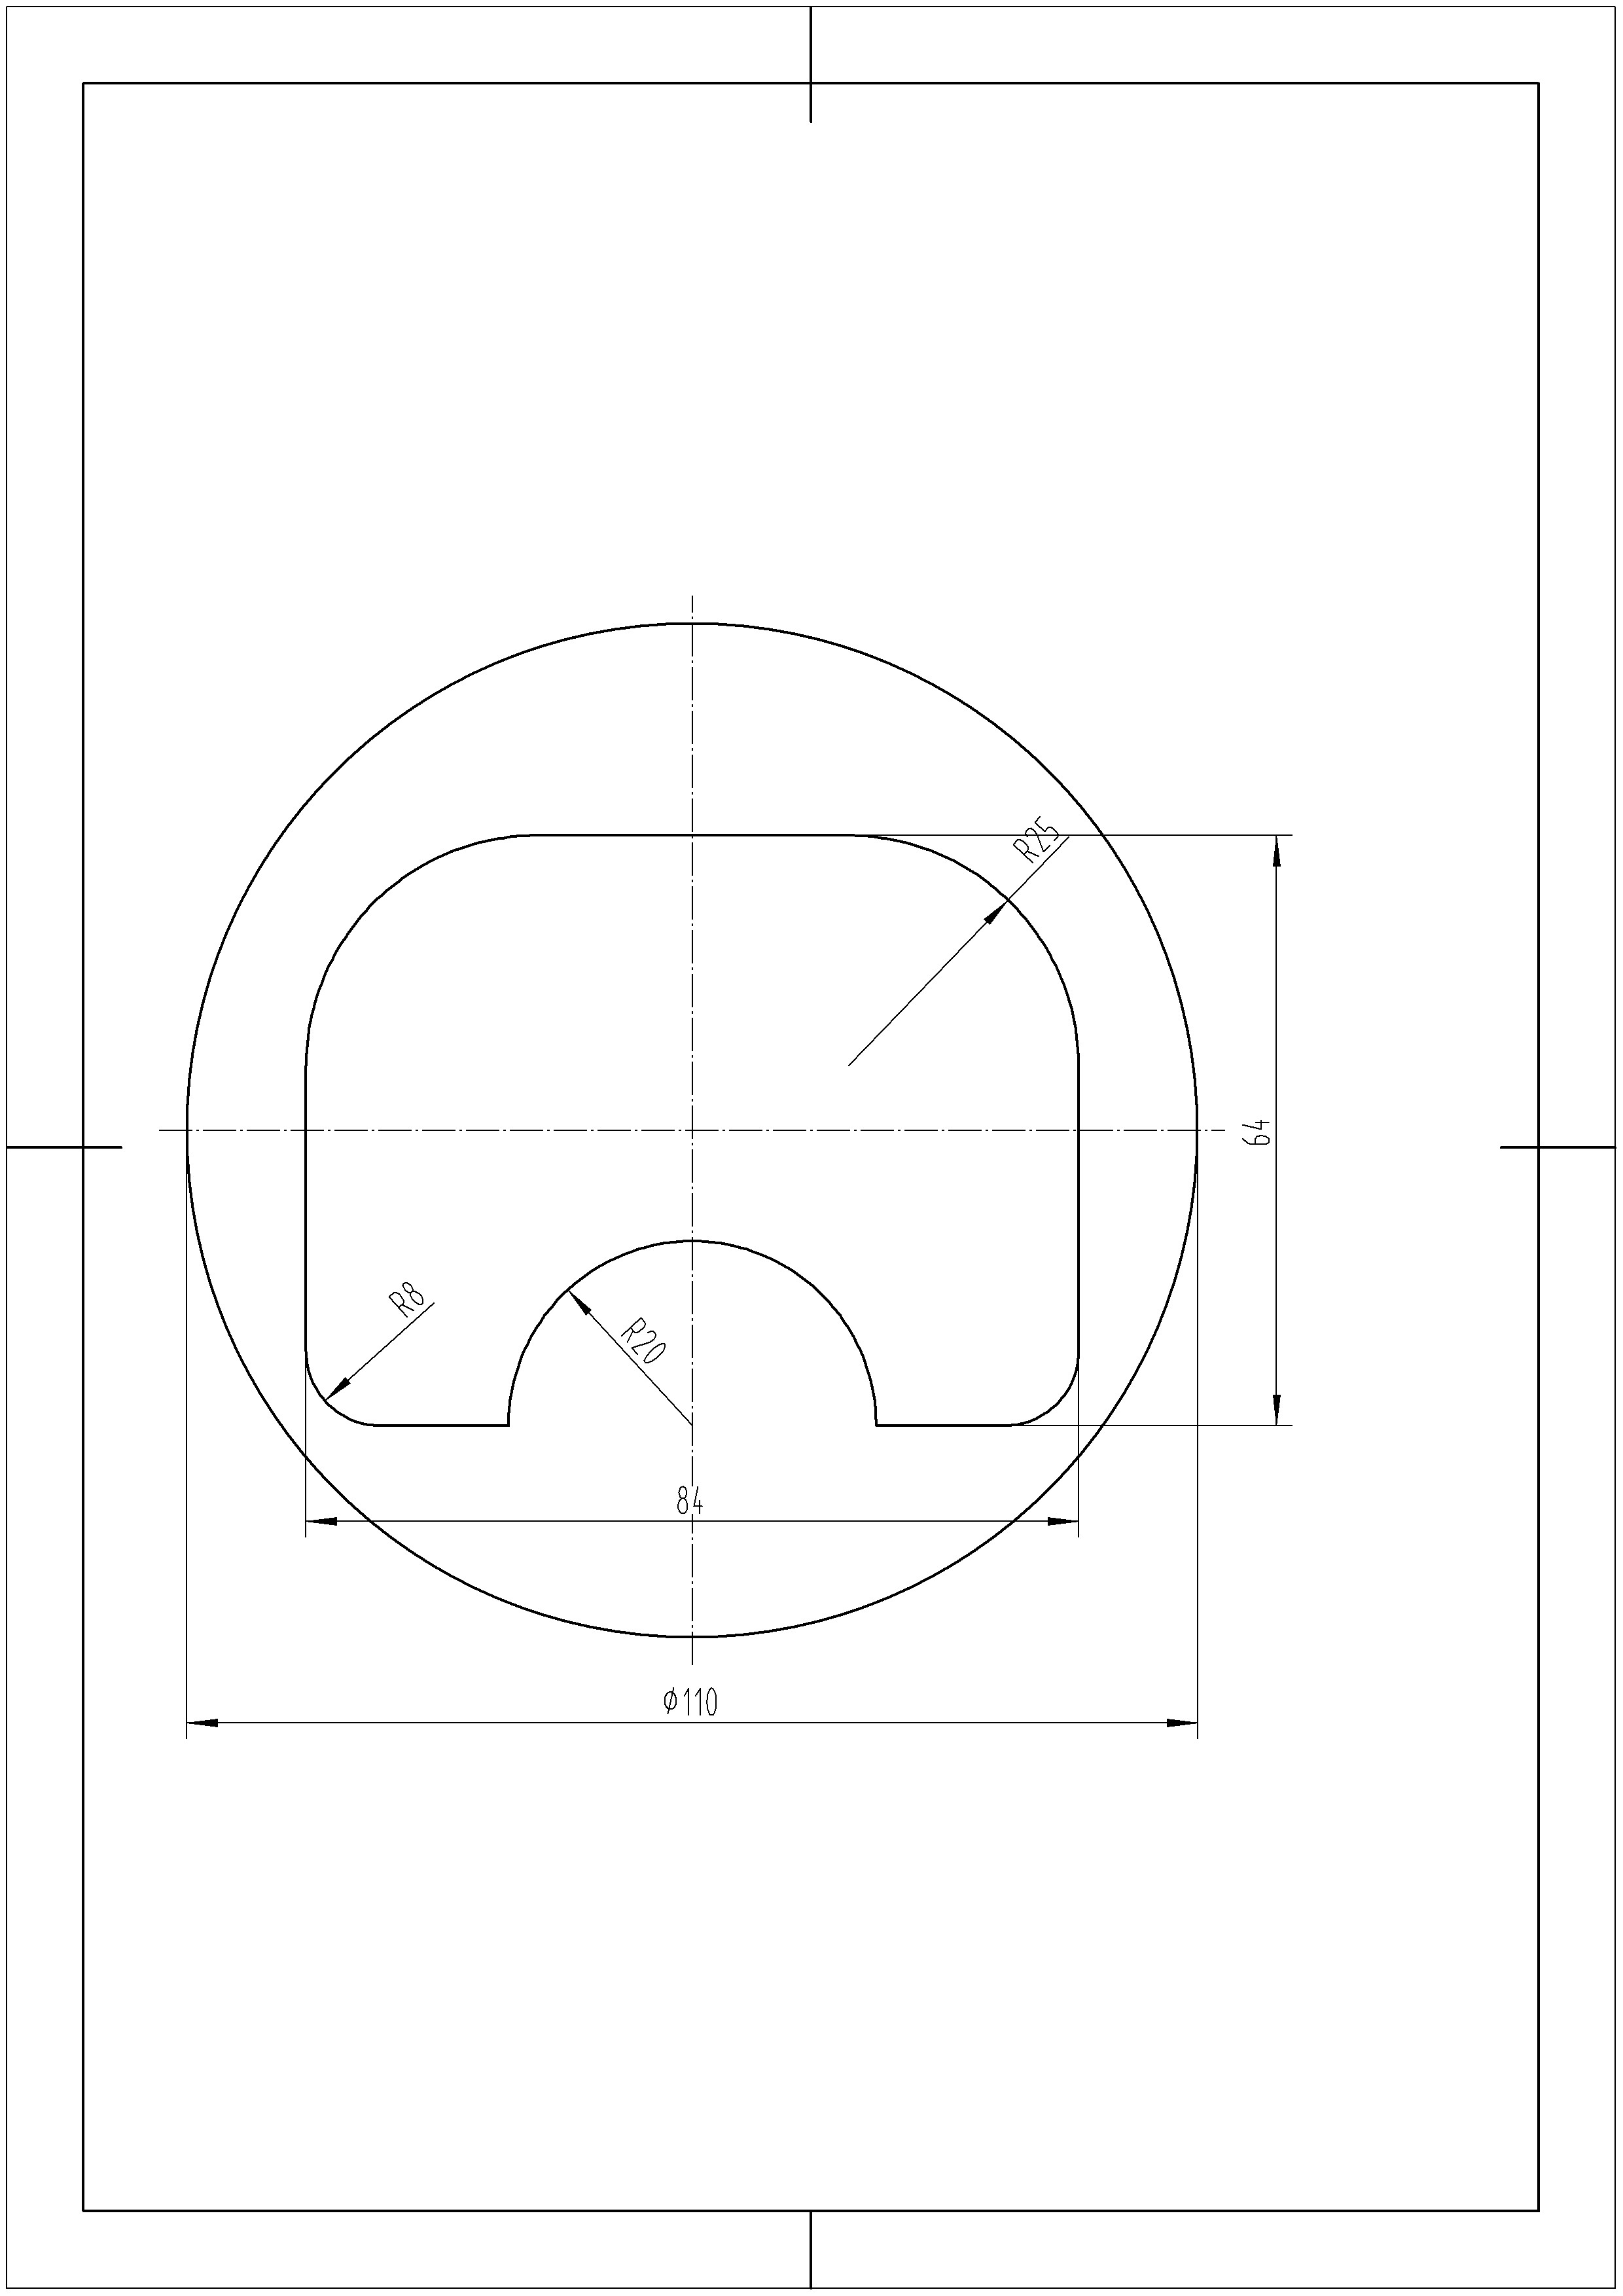
\includegraphics[width=0.8\linewidth,trim=40 150 70 220,clip]{data/image/7-2.jpg}
	\caption{复习实例2}
	\label{fig:8-1}
\end{figure}
\end{enumerate}


\subsection{教学内容及过程}

\subsubsection{刀具半径补偿}

由CNC系统内部使刀具在加工时,自动偏移一个刀具半径。
简化编程的难度。

指令G40、G41/G42

1、补偿方向的确定:

ISO 标准规定,当刀具中心轨迹在编程轨迹前进方向的左边时,称为左刀补,用G41表示;刀具中心轨迹在编程轨迹前进方向的右边时,称为右刀补,用G42表示;注销刀具半径补偿时用G40表示。

\begin{figure}[h]
	\centering
	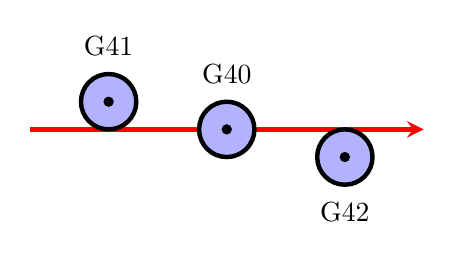
\begin{tikzpicture}[ultra thick]
	\draw[->,red,>=stealth]  (0,0) -- (5,0);
	\draw[fill=blue!30] (1,10pt) circle (10pt) circle (1pt);
	\draw[fill=blue!30] (2.5,0) circle (10pt) circle (1pt);
	\draw[fill=blue!30] (4,-10pt) circle (10pt) circle (1pt);
	\node at (1,30pt) {G41};
	\node at (2.5,20pt) {G40};
	\node at (4,-30pt) {G42};
	\end{tikzpicture}
	\caption{刀补位置}
	\label{fig:8-1}
\end{figure}

2、补偿值的设定:

通过参数进行设定:

[OfFset]---[补偿]----[位置号]----[D形状+D磨shen损]

3、指令的格式:

在开始刀补的位置,结合G1指令设定补偿方向及补偿值位置号,在结束的位置,用G40结合G1指令即可:

G41/G42 G1 X\_ Y\_  D\_;

……

G40 G1 X\_ Y\_;

4、补偿平面

可以在G18及G19平面上进行刀具半径补偿,(常用于球头刀)

5、补偿过程分析:

1)刀具半径补偿建立:当输入BS缓冲器的程序段包含有G41/G42命令时,系统认为此时已进入刀补建立状态。当以下条件成立时,加工中心以移动坐标轴的形式开始补偿动作。 

a. 有G41或G42被指定; 

b. 在补偿平面内有轴的移动; 

c. 指定了一个补偿号或已经指定一个补偿号但不能是D00;

d. 偏置(补偿)平面被指定或已经被指定; 

e. G00或G01模式有效。 

2) 补偿模式:在刀具补偿进行期间,刀具中心轨迹始终偏离编程轨迹一个刀具半径值的距离。此时半径补偿在G00、G01、G02、G03情况下均有效。 

3) 取消补偿:使用G40指令消去程序段偏置值,使刀具撤离工件,回到起始位置,从而使刀具中心与偏程轨迹重合。当以下两种情况之一发生时加工中心补偿模式被取消。

①给出G40同时要有补偿平面内坐标轴移动。

②刀具补偿号为D00。

4)不同平面内的半径补偿 

刀具半径补偿用G17、G18、G19命令在被选择的工作平面内进行补偿。即当G18命令执行后,刀具半径补偿仅影响X、Z移动,而对Y轴没有作用。


\subsubsection{注意事项}
1、G41/G42必须与G1/G0结合使用,不可在G2/G3圆弧指令下使用。

2、刀具必须在加工平面内有移动。

3、使用与取消必须成对使用。

4、加工前必须设定其补偿值。

5、切入前指定、切出后取消。

\subsubsection{加工实例}
毛坯:φ110*35

刀具:φ12立铣刀

加工路径:如图\ref{fig:8-2}所示:

\begin{figure}[h]
	\centering
	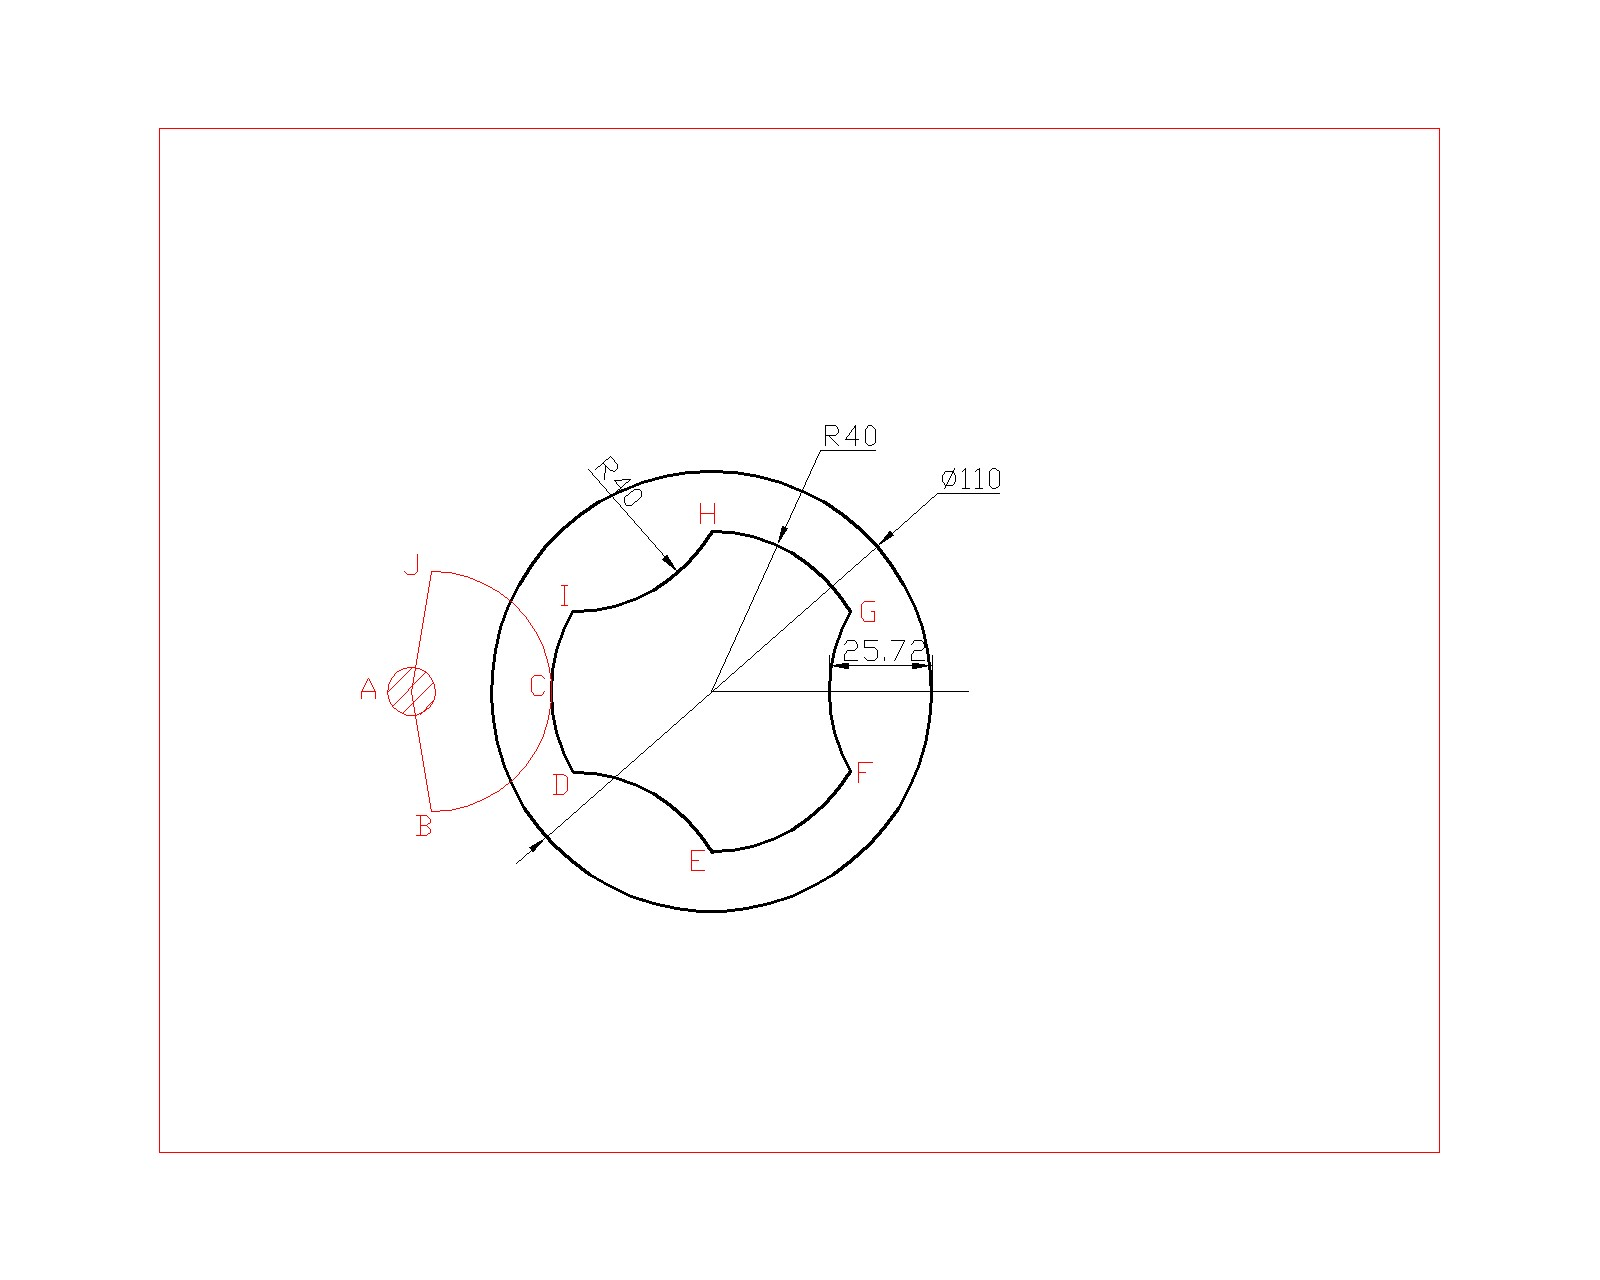
\includegraphics[width=0.8\linewidth,trim=280 250 430 280,clip]{data/image/8-2.jpg}
	\caption{刀补实例}
	\label{fig:8-2}
\end{figure}

参考程序:
\begin{lstlisting}
G54G17G40G49G90
M03 S300
G0 X-70.0 Y0
Z5.0
G01 Z-5.0 F500
G41 G01 X-60 Y-20 D01
G03 X-40.0 Y0 R20.0
G02 X-34.641 Y20.0 R40.0
G03 X0 Y40.0 R40.0
G02 X34.641 Y20 R40.0
G03 Y-20.0 R40.0
G02 X0 Y-40.0 R40.0
G03 X-34.641 Y-20 R40.0
G02 X-40 Y0 R40.0
G03 X-60 Y0 R20.0
G40 G01 X-70 Y0
G0 Z30
M05
M30
\end{lstlisting}

\subsubsection{刀具半径补偿值的确定}

1、粗加工:

为半精/精加留余量:0.2-0.6 (单边)

Offset=D/2+余量

2、半精加工:

为精加留余量:0.1-0.2 (单边)

Offset=D/2+余量

3、精加工:

Offset= Offset (上次)+修正

修正=(理论值-测量值)双边/2 

4、处多余材料:

Offset值不能太大



\subsection{课堂小结}
\begin{enumerate}[1、]
\item 刀补的概念
\item G40、G41/G42指令的使用;
\item 注意事项;
\item 刀补的编程;
\item 刀补值的计算。
\end{enumerate}

\vfill
\subsection{布置作业}
\begin{enumerate}[1、]
	\item 写出上面的程序。
\item 习题集。
\end{enumerate}
\vfill